\documentclass[11pt]{article}
\usepackage{hyperref}
\usepackage{sectsty}
\usepackage{graphicx}
\usepackage{amssymb}
\usepackage{indentfirst}

\hypersetup{
    colorlinks=true,
    linkcolor=blue,
    filecolor=magenta,      
    urlcolor=cyan,
    pdftitle={Overleaf Example},
    pdfpagemode=FullScreen,
}

% Margins
\topmargin=-0.45in
\evensidemargin=0in
\oddsidemargin=0in
\textwidth=6.5in
\textheight=9.0in
\headsep=0.25in

\title{Exercício para sala de aula - Árvores de decisão e Ensembles}
\author{ João Paulo Mota }
\date{\today}

\begin{document}
\maketitle

% Optional TOC
% \tableofcontents
% \pagebreak

%--Paper--

\section{Roteiro do exercício}

\subsection{Exercício 1 - Treinamento do modelo baseado em árvore de decisão}
O treinamento do modelo de árvore de decisão foi feito utilizando a biblioteca GridSearchCV para busca de melhores parâmetros.
Sabemos que a qualidade dos candidatos a split de um nó e, por consequência, a escolha feita pelo modelo em treinamento  como dividir o nó, é feita analisando 
funções de impureza ou de perda.
Aqui analisamos log\_loss, gini impurity e entropy. Os resultados foram:

\begin{itemize}
  \item criterion=log\_loss, precision=0.8861, training\_time=0.1876, max\_depth=None
  \item *criterion=entropy, precision=0.8861, training\_time=0.1848, max\_depth=None
  \item criterion=gini, precision=0.8416, training\_time=0.0960, max\_depth=None
\end{itemize}

Note que escolhemos não setar uma profundidade máxima pois o dataset é relativamente pequeno e é vantajoso que o modelo continue fazendo splits até que todas as folhas sejam puras (pertençam a uma só classe).

Abaixo vemos a matrix de confusão e a árvore resultando para os parâmetros escolhidos (linha marcada com *)
\\
\begin{center}
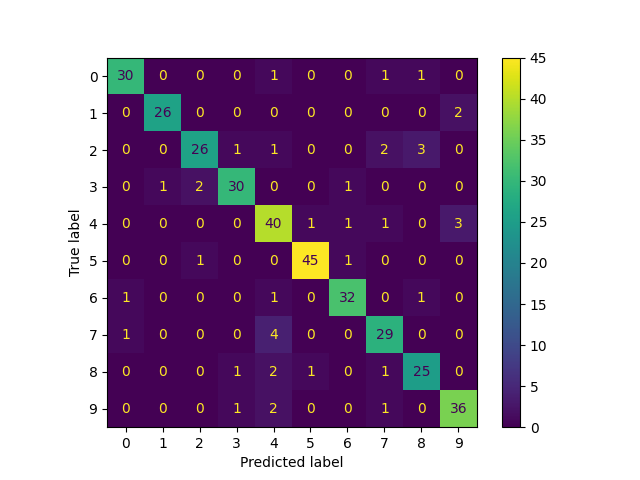
\includegraphics[height=0.28\textheight]{decision_tree_confusion_matrix.png}
\\
\includegraphics[height=0.28\textheight]{decision_tree_plot.png}
\end{center}

\subsection{Exercício 2 - Avaliação dos ganhos com a utilização de modelos Ensemble}
Vemos um ganho substancial de performance utilizando modelos Ensemble.

Abaixo vemos dados de análise dos modelos Ensemble utilizados:

Random Forest:
\begin{itemize}
  \item criterion=log\_loss, precision=0.9701, training\_time=0.1876, max\_depth=None
  \item *criterion=entropy, precision=0.9722, training\_time=0.1848, max\_depth=None
  \item criterion=gini, precision=0.9722, training\_time=0.0960, max\_depth=None
\end{itemize}

XGBoost:
\begin{itemize}
  \item max\_depth=5, training\_time=1.5073583126068115, precision=0.9666666666666667 
  \item *max\_depth=10, training\_time=1.6833817958831787, precision=0.9694444444444444
  \item max\_depth=100, training\_time=1.5776081085205078, precision=0.969444444444444 
  \item max\_depth=1000, training\_time=1.555584192276001, precision=0.9694444444444444
\end{itemize}

\subsection{Exercício 3 - Visualização da árvore de decisão e Medida de Impureza}
Olhar items anteriores.

\subsection{Exercícios 4, 5 e 6}
Ver código python que acompanha esse relatório e arquivo README

%--/Paper--

\end{document}
